\documentclass[a4paper, 11pt, nofootinbib]{book}

\setcounter{tocdepth}{3}
\setcounter{secnumdepth}{3}
\usepackage{amsmath}
\usepackage{comment} % enables the use of multi-line comments (\ifx \fi) 
\usepackage{lipsum} %This package just generates Lorem Ipsum filler text. 
\usepackage{fullpage} % changes the margin
\usepackage[utf8]{inputenc}
\usepackage{gensymb}
\usepackage{graphicx}
\usepackage{booktabs}% http://ctan.org/pkg/booktabs
\usepackage{makecell}
\usepackage{tabularx}
\usepackage[table]{xcolor}
\usepackage{array}
\usepackage{wrapfig}
\usepackage{subcaption}
\usepackage{csquotes}
\usepackage{lscape}
\usepackage{afterpage}
\usepackage{geometry}
\usepackage{listings}
\usepackage{xcolor}
\usepackage{ulem}
\usepackage{chngcntr}
\usepackage{multicol}

%Tabellenheadings
\renewcommand*{\thead}[1]{\bfseries #1}

%Ermöglicht bullet-points in Tabellen
\newcommand \tabitem{\makebox[1em][r]{\textbullet~}}

%Abbildungen werden pro Kapitel nummeriert (Abb. 1.4, Abb. 4.7 etc)
\counterwithin{figure}{section}

\geometry{a4paper, margin=1in}

%Bilder haben die Unterschrift Abb. anstelle von Figure
\renewcommand{\figurename}{Fig..}

%\code{Text} formatiert Text als monospace Schrift
\newcommand{\code}[1]{\texttt{#1}}


%Wie sollen Code-Snippets mit \lstinline|code| aussehen?
\lstset{frame=tb,
	language=c,
	aboveskip=3mm,
	belowskip=3mm,
	showstringspaces=false,
	columns=flexible,
	basicstyle={\small\ttfamily},
	numbers=none,
	numberstyle=\tiny\color{gray},
	keywordstyle=\color{blue},
	commentstyle=\color{darkgreen},
	stringstyle=\color{violet},
	breaklines=true,
	breakatwhitespace=true,
	tabsize=3
}

%RGB-Definition von eiigen Farben
\definecolor{system}{RGB}{141,0,76}
\definecolor{inhalt}{RGB}{2,47,99}
\definecolor{darstellung}{RGB}{116,117,117}
\definecolor{nutzung}{RGB}{207,2,127}
\definecolor{darkgreen}{RGB}{39,117,1}

\begin{document}
\title{Summary Micro-Controller FS18}
\author{Alex Neher}
\maketitle

\tableofcontents

\graphicspath{{./Pictures/}}

\mainmatter
\chapter{Microcontroller}
\section{Components}
Micro controllers are so called \textbf{Single Chip} Computer, meaning everything is on a single PCB, as opposed to e.g. a 'normal' PC.

\begin{wrapfigure}[8]{R}{0.5\textwidth}
	\centering
	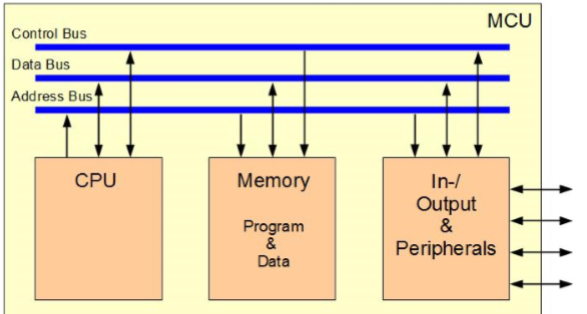
\includegraphics[keepaspectratio=true,height=10\baselineskip]{architecture.PNG}
	\caption{Von-Neumann Architecture}
	\label{fig:arch}
\end{wrapfigure}

MC consist of at least four components:

\begin{description}
	\item[CPU: ] Central Processing Unit
	\item[Memory: ] Where programs and data are stored
	\item[IO/Input-Output: ] Communication with Peripherals
	\item[Bus-System: ] Connects the components
\end{description}

\vspace{10px}

\noindent There are two different architectures:

\begin{description}
	\item[Von-Neumann: ] One shared bus for program and data. Program and data are in the same memory. Often found in low-cost MCs
	\item[Harvard: ] Two separate bus systems for program and data. Often found in high-performance MCs
\end{description}
\vspace{10px}

\noindent Usually, a read/write-operation goes through four steps:

\begin{enumerate}
	\item CPU puts the address on the address bus
	\item Either the memory or the IO claim the address as their
	\item CPU tells the component via the control bus whether the operation is read or write
	\item 
		\subitem \textit{read: } The memory or IO places the data of the requested address on the data bus
		\subitem \textit{write: } The CPU writes the data on the mentioned address via data bus
\end{enumerate}

\section{Numerical systems}
In MC, variables and constants are seldom stored as decimal value. Rather they're either stored as a binary or a hexadecimal value. 

In general, mathematical terms an $n$-digit integer to the base $B$ can be expressed as:

\[ \scalebox{1.5}{$ \sum_{i=0}^{n-1} x_{i} * B^i = X_{0} * B^0 + x_{1} * B^2 + [...] + x_{n-1} * B^{n-1} $} \]

\noindent Or easier: \textit{Multiply the $n$-th digit of the integer with $B^{n-1}$ starting from the right} with n = 0

\subsection{Example}

\noindent $1100'0101_{2}$ (binary) to decimal \\
$
	= 1*2^0 + 0*2^1 + 1*2^2 + 0*2^3 + 0*2^4 + 0*2^5 + 1*2^6 + 1*2^7 \\
	=   1   +   0   +   4   +   0   +   0   +  0   +   64   +  128 \\
	=   \underline{\underline{197_{10}}}
$

\noindent If you have to convert a number between two 'exotic' systems, say base 8 to base 3, it's usually easier to convert it to decimal first and then convert it to the desired system again ($x_{8} \rightarrow x_{10} \rightarrow x_{3}$). An exception to that is binary to hexadecimal and vice versa. One digit in hexadecimal represents four digits in binary, so you can directly convert blocks of four:

\noindent $1100'0101_{2}$ to hexadecimal:
\vspace{10px}

\noindent
$1100 = 0*2^0 + 0* 2^1 + 1*2^2 + 1*2^3 = 0 + 0 + 4 + 8 = 12_{10} = C_{16} \\
0101 = 1 * 2^0 + 0*2^1  + 1*2^2 + 0*2^3 = 1 + 0 + 4 + 0 = 5_{10} = 5_{16} \\
\rightarrow 1100'0101_{2} = C5_{16}
$

\subsection{Two's Complement}
Especially in MC-technology, signed numbers (that can also be negative) are mostly stored as \textit{two's complement}. You basically take the binary number, invert every digit and add one. So -28 would be stored as
\vspace{10px}

\noindent
$ 28_{10} = 16 + 8 + 4 = 2^2 + 2^3 + 2^4 = 0001'1100_{2}$ \\
invert \\
$ 0001'1100 \rightarrow 1110'0011$\\
add one \\
$1110'0011 + 1 = \underline{\underline{1110'0100}}$

\section{Logic Gates}
\begin{figure}[htb]
	\centering
	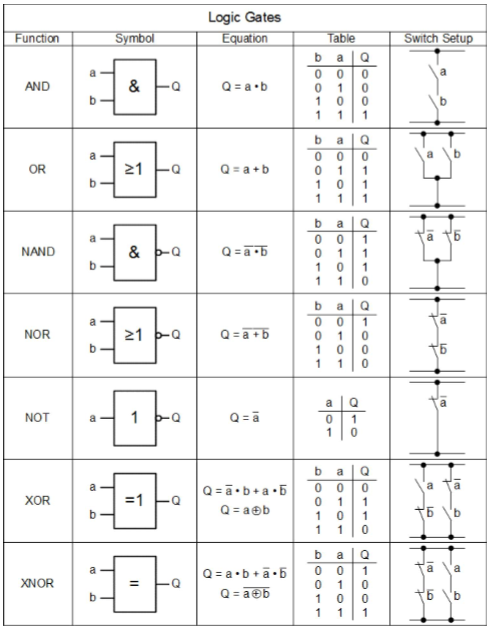
\includegraphics[keepaspectratio=true,height=25\baselineskip]{logicGates.PNG}
	\caption{Fundamental logic-Gates used in MCs}
	\label{fig:logicGates}
\end{figure}

\begin{figure}[htb]
	\centering
	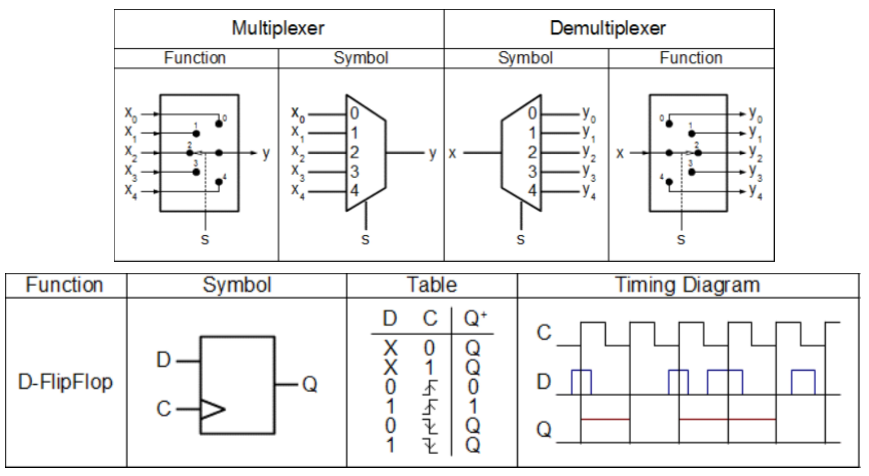
\includegraphics[keepaspectratio=true,height=15\baselineskip]{flipflop.PNG}
	\caption{Visualisation of the (de)multiplexer and the flipflop}
	\label{fig:multFlip}
\end{figure}

\begin{description}
	\item[Multiplexer: ] The multiplexer is a combinational logic circuit, which allows us to select one of many input lines and route it to the single, common output line. The demultiplier does the exact opposite: it takes one input and you can select to which output line it is routed
	\item[FlipFlop: ] Idunno %TODO
\end{description}

\section{Instruction Set Cycle}

\begin{wrapfigure}[7.5]{L}{0.5\textwidth}
	\centering
	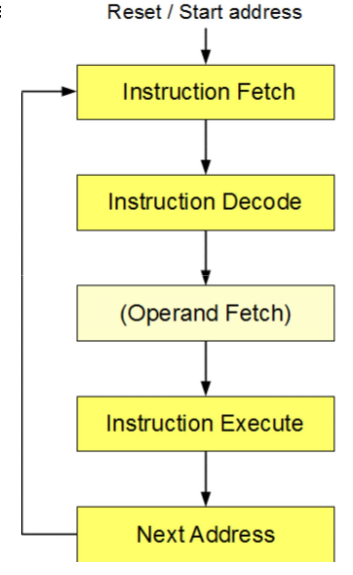
\includegraphics[keepaspectratio=true,height=20\baselineskip]{instructionCycle.PNG}
	\caption{Visualisation of the Instruction Set Cycle}
	\label{fig:instCycle}
\end{wrapfigure}

The way a CPU executes instructions can be shortened to \textbf{FDE}. It stands for \textbf{F}etch, \textbf{D}ecode \textbf{E}xecute. 
\vspace{10px}
S
\noindent As can be seen in fig. \ref{fig:instCycle}, the CPU first fetches the instruction from the memory, then it decodes it and decides if it has to fetch a second operand (e.g. for an addition). Afterwards it executes said instruction and moves on to the next address.


\newpage

\section{Assembler}
\subsection{Directives}
Put simply, Assembler directives are instructions that direct the assembler to do something:
\begin{center}
\begin{tabular}{|p{2cm}|p{5cm}|p{4cm}|p{5cm}|}
	\hline
	\thead{Directive} & \thead{Description} & \thead{Example} & \thead{Explanation} \\
	\hline
	SECTION & Defines the beginning of a relocatable section & ConstSec: SECTION & Puts the whole ConstSec-Section in the same RAM-section\\
	\hline
	EQU & Assign an expression to a name. Not redefinable & MaxElement: EQU 20 & search-and-replace every \textit{MaxElement} in the code with 20\\
	\hline
	DC & Defines one or more constants and theirnames & DC B \$AA & Pointer to address \$AA at every \textit{Alarm}\\
	\hline
	DS & Allocates memory to variables & DS W 3 & Reserves 3 words of RAM. 1 Word = 2 Bytes\\
	\hline
\end{tabular}
\end{center}

\subsection{Addressing modes}
There are six different addressing modes that are supported by our CPU:

\begin{description}
	\item[Immediate: ] 1 Byte operand in the instruction \\
		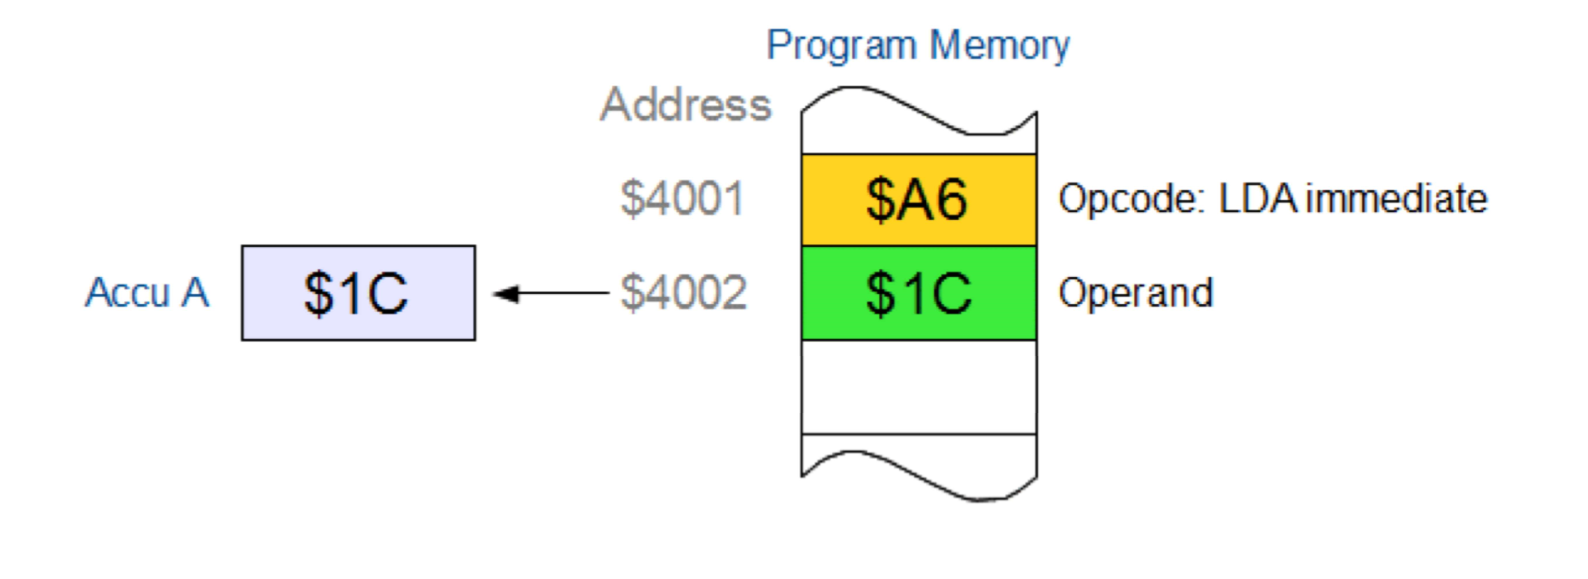
\includegraphics[keepaspectratio=true, height=10\baselineskip]{immAdd.PNG}
	\item[Inherent: ] No operand required \\
		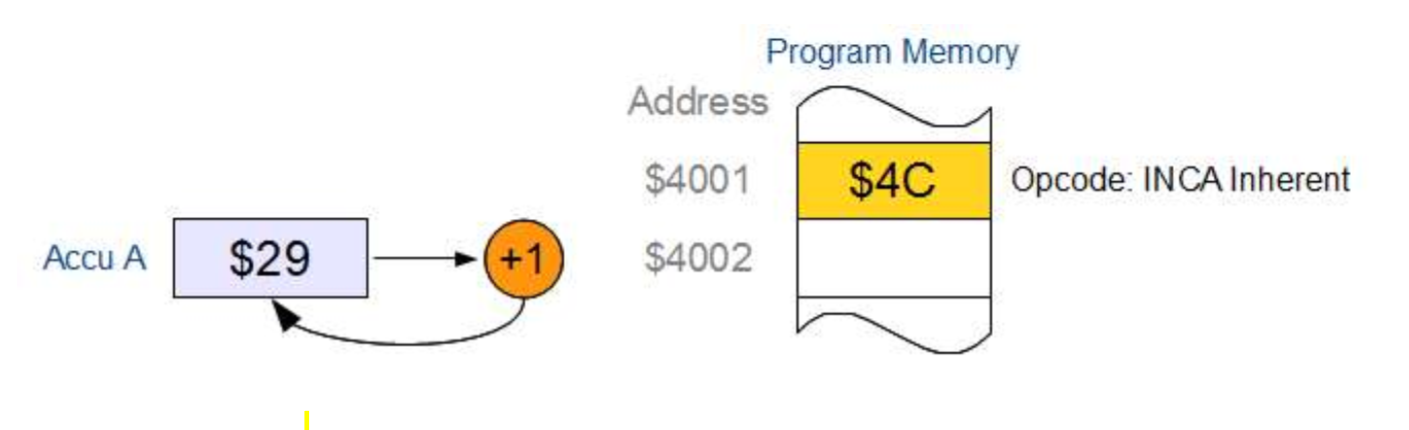
\includegraphics[keepaspectratio=true, height=10\baselineskip]{inhAdd.PNG}
	\item[Direct: ] Operands must be stored in the Direct Page (From \code{0x0000} to \code{0x00AF}) \\
		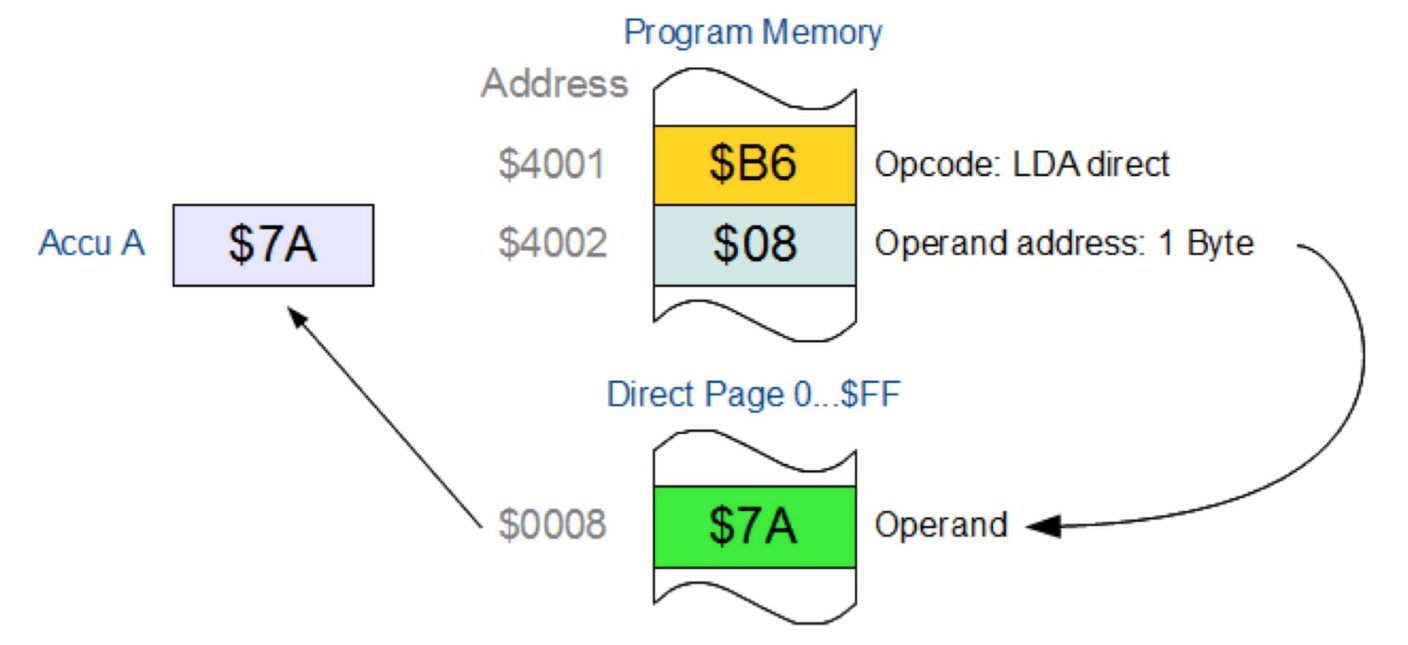
\includegraphics[keepaspectratio=true, height=10\baselineskip]{dirAdd.PNG}
	\item[Extended: ] Operand can be stored in the whole 64k Memory \\	
		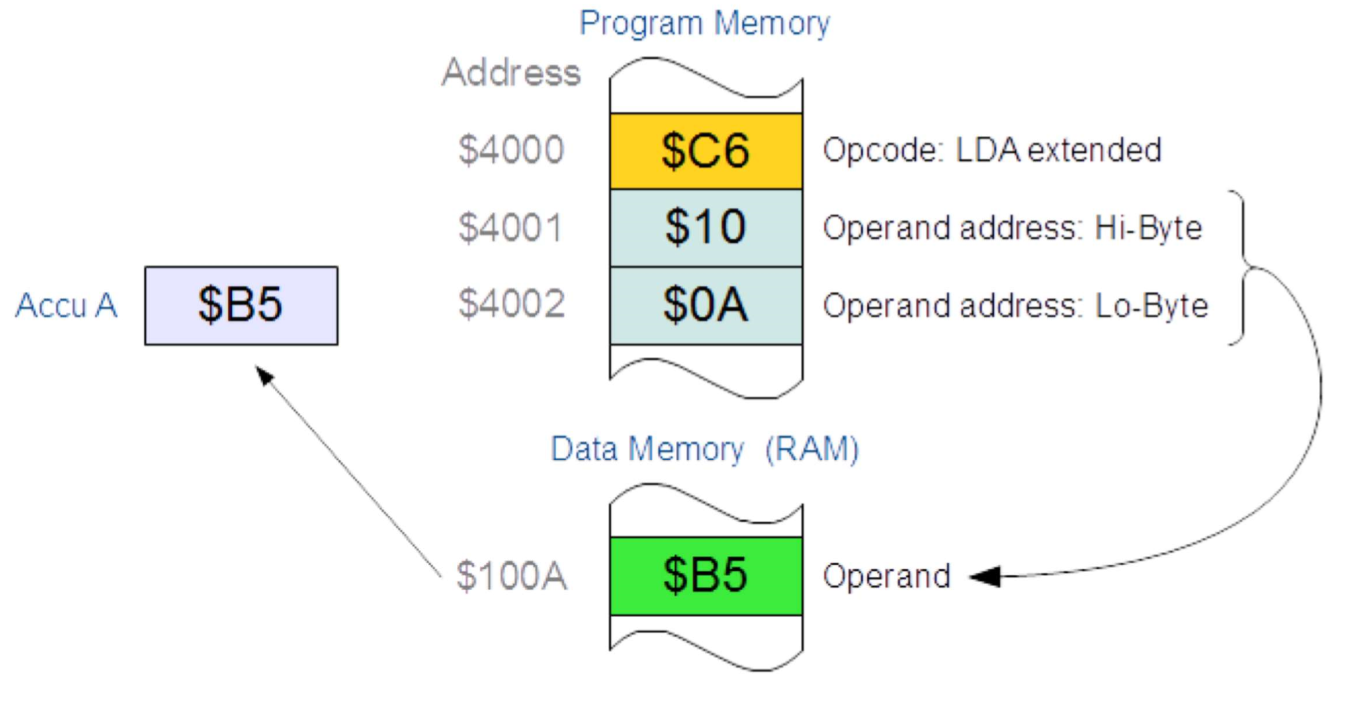
\includegraphics[keepaspectratio=true, height=10\baselineskip]{extAdd.PNG}
	\item[Indexed: ] Operand is stored in Stack Pointer or H:X Register \\
		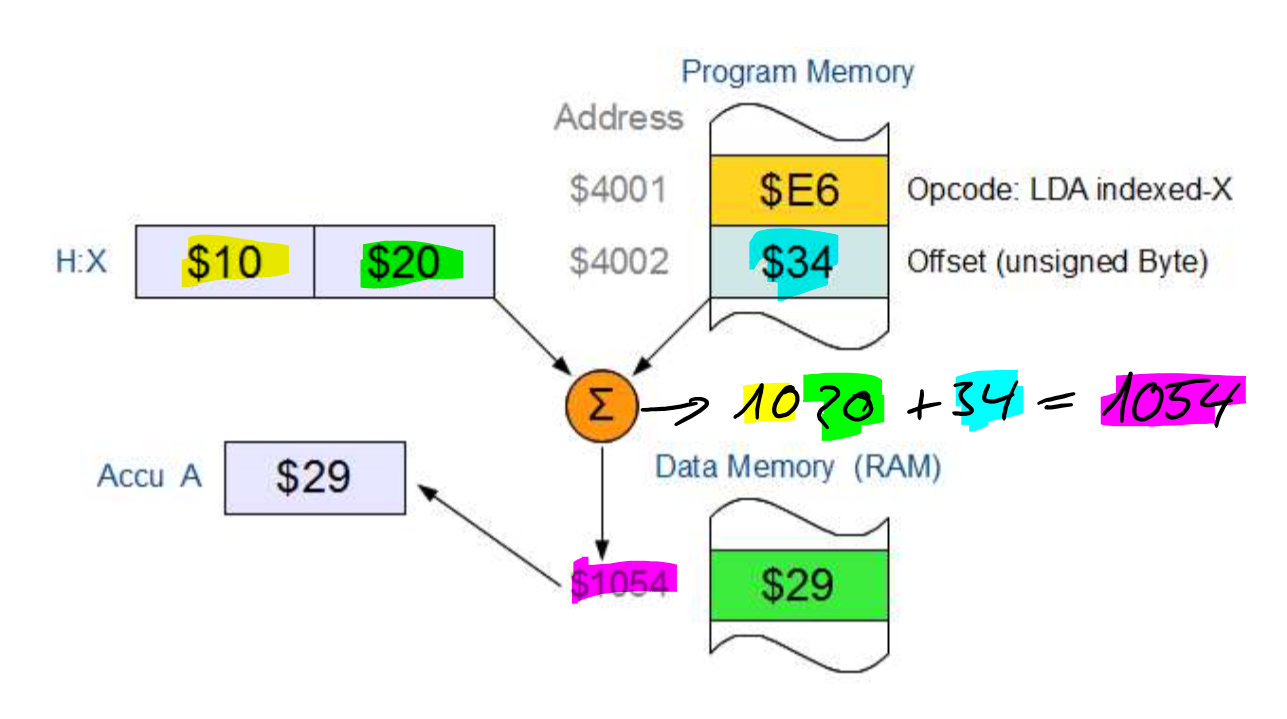
\includegraphics[keepaspectratio=true, height=10\baselineskip]{indAdd.PNG}
	\item[Relative: ] Only used with \code{BRANCH}-Instructions. Depending on outcome of the Branch \\
		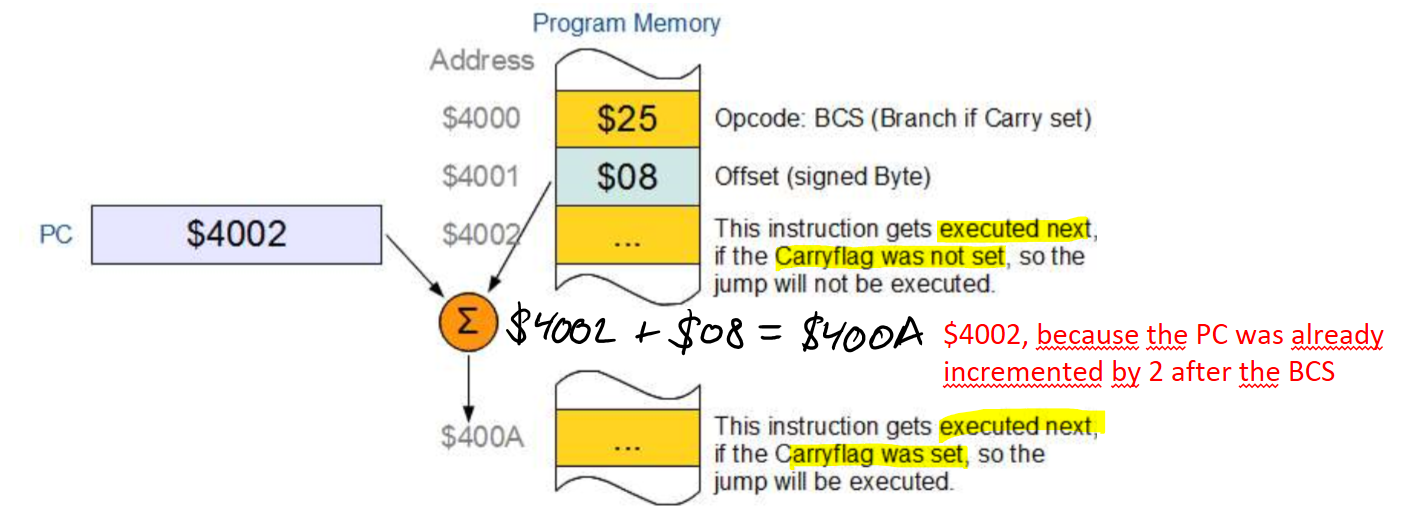
\includegraphics[keepaspectratio=true, height=10\baselineskip]{relAdd.PNG}
\end{description}

\newpage

\subsection{Assembler Programming Operations}
There are three main assembler instruction types:

\begin{itemize}
	\item Data Transport
		\subitem Load
		\subitem Store
		\subitem Transfer
		\subitem Move
	\item Operations
		\subitem Arithmetic
		\subitem Logic
		\subitem Bit-Manipulation/Masking
		\subitem Shift and Rotation
	\item Branching
\end{itemize}

\subsubsection{Data Transport}
Data Transport instructions are again divided into four subtypes

\begin{figure}[htb!]
	\centering
	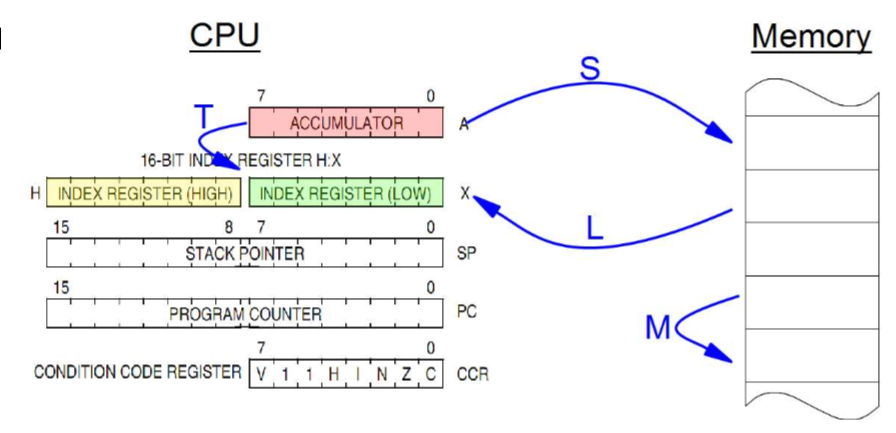
\includegraphics[keepaspectratio=true,height=15\baselineskip]{assOperations.PNG}
	\caption{Visualisation of the different data tranfers}
	\label{label}
\end{figure}

\begin{description}
	\item[Load: ] Data is moved from the memory to the CPU-Register \\
		Examples: \code{LDA, LDX, LDHX, (PULA, PULX} Stack-operations)
	\item[Store: ] Data is moved from the CPU-Register to the memory \\
		Examples: \code{STA, STX, STHX, (PSHA, PSHA} Stack-operations) 
	\item[Transfer: ] Very fast Data Transfer between CPU registers
		Examples: \code{TAP, TPA, TAX, TSX}
	\item[Move: ] Data is moved within the memory
\end{description}



\chapter{C}

\end{document}
